\chapter{Tasks and Methods}
\label{TaskAndMethods}
The purpose of the following chapter is to answer the research question presented in \autoref{ResearchQuestion} by proposing tasks for the development of the TonePrint community, in which the involvement of users is considered beneficial. The tasks are proposed on the basis of the results of the Thematic analysis and the Conceptual model described in \autoref{CommunityConcept}, and they focus on how to acquire the necessary information from the users to design content in the TonePrint community. The descriptions of these tasks will include relevant methods, and how they may be employed best to the design process of TC Electronic. This is done on the basis of their SCRUM framework and from personal experience with utilizing these methods. After outlining the possible tasks and subsequent methods to engage with, one of them will be chosen to be investigated in this project.

%Define the task - What is the goal?
%How can this be investigated? - Which methods can be applied for it?
%What is the realistic time aspect for applying these methods? How long do they take? / How are they best applied for the design process at TC Electronic? (SCRUM)
%%What equipment and how many subjects are required?

\section{Task 1: Designing the information architecture}
\label{Task1}
When designing the TonePrint community, it's important to consider the structure of the information, better known as information architecture. The purpose of this is to ensure that the design accommodates the users' understanding of the system in terms of being a closer match to the conceptual model of the system. This would ease the use of the system, as the system would act accordingly to the users' expectations. As explained in Chapter 4, TC Electronic haven't acquired information about their users understanding of the TonePrint application before, which makes this task even more important. two ways of approaching this will be addressed. \\

\noindent
One approach could be to involve the users early on while designing the system by letting them take part in shaping the concept and flow of the community. This is also referred to as a \textit{participatory design procedure} \parencite{PDF:ParticipatoryDesignMethods}. During this, the users are provided a chance of influencing the design of a future product for example by conducting workshops with them as participants. In the case of the TonePrint community, these workshops could for example be set up with multiple steps focusing on different aspects of the information architecture. This could include a brainstorming session for creating conceptual ideas for the community, a card sorting task where these ideas are grouped, and a session for creating prototypes from these groups. Another approach also focusing on the information architecture could be to test the current thoughts and ideas of how the application should be structured through prototype testing. prototyping comes to mind in this context, either in the the shape of low-fidelity or high-fidelity prototypes \parencite[][228]{PDF:DonNorman}. These are used to test the functionality of an application, even though a finished version of the product isn't available. For low-fidelity prototypes, these mock-ups are instead constructed from easy accessible materials without spending much time on the aesthetic appearance, while high-fidelity are closer to a finished product. For the TonePrint community, lo-fi prototyping can be employed to indicate how the functionalities and features shall be shaped, early on, through user tests with the information architecture in focus. This makes lo-fi prototyping very useful to employ, however, they require a rough idea of how the system should work and how the information is going to presented before conducting the actual test. When brainstorming possible methods for testing with lo-fi prototypes, \textit{the cognitive walkthrough} comes to mind as a suitable suggestion \parencite{WEB:CognitiveWalkthrough}. Through this method, the subjects are given a number of tasks to complete on the prototype, where each task has a well defined action sequence necessary to follow step-by-step, in order complete the task correctly. The subjects' results are then analysed through general principles of cognitive psychology in order to locate potential pitfalls in the design.\\

\noindent
For either of the tasks above, some planning and preparation is necessary. firstly in the case of constructing lo-fi prototypes, the necessary materials are needed to create a fitting representation. For a participatory design workshop, there are some materials required depending on the sessions in the workshop, but in general, generic elements such as post-it notes and pens for the brainstorming session are needed. The subjects required for participating, whatever the approach, need to account for the possible end-users of the TonePrint community, which means musician familiar with the TonePrint concept. Other groups could also be represented, depending on the scope of the study. If it's of interest, TonePrint users could be employed in comparison with sound engineers or maybe even novices. The process of acquiring the subjects can be eased with the help of TC Electronic themselves though their existing online communities. For the cognitive walkthrough the subjects don't necessarily require the same level of background knowledge, as it can be conducted with novices and experts alike, depending on the chosen approach \parencite{WEB:CognitiveWalkthrough}. As such, the members of the development teams at TC Electronic could also be used as subjects for the test.\\

\noindent
From personal experience of previous semester projects utilizing some of these methods, fitting them to a 3-week sprint is considered fairly doable. As already mentioned, the methods require some planning, and with an employee dedicated to this phase, the appropriate amount of time can be applied to it. \autoref{fig:SprintFitExample} illustrates a graphical proposal to how it can fit to the SCRUM framework, where each sprint is divided into weekly intervals. Each of these weeks focuses on the different parts of conducting user studies, \textit{planning}, \textit{execution}, and \textit{analysis}. As it appears from the figure, it's furthermore proposed to combine the analysis phase for one sprint with a \textit{pre-planning} phase for the next. This is not intended to add further workload to an already important phase of the sprint, but the employee dedicated to conducting the studies would benefit from making some early thoughts of the sprint to come, easing the actual planning phase. This is especially considered beneficial, if the individual sprints represent minor user tests contributing to one overall scope. By the end of each sprint, the results of the test are presented to the rest of the development team during \textit{sprint demos} similarly to the other members.
%
\begin{figure}[H]
	\centering
	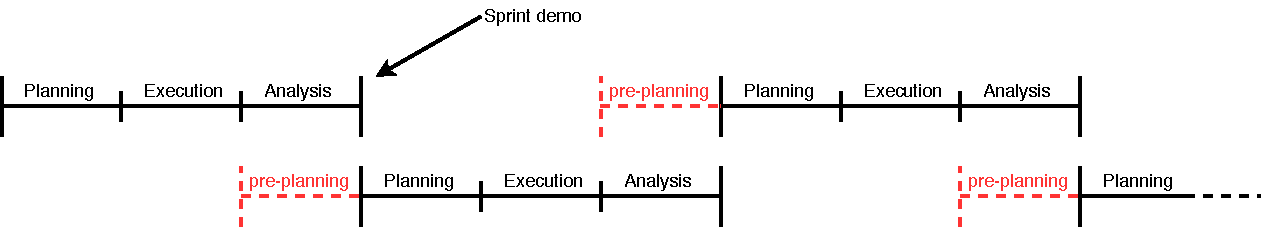
\includegraphics[width=\textwidth]{SprintFitExample.pdf}
	\caption{An illustration of how to fit minor user studies to the SCRUM framework. Each sprint period is split into weekly intervals with the final week also functioning as a pre-planning phase for the next sprint.}
	\label{fig:SprintFitExample}
\end{figure}


\section{Task 2: Tags}
\label{Task2}
A new feature for the TonePrint community is \textit{tagging}, which was a prominent topic during the interview, see \autoref{ThematicFindings}. Aiding the users in categorising and in general getting a better overview of the potentially many User TonePrints is considered important by TC, and proposals should therefore be made to a study with this in focus. Choosing an approach for this requires some clarification to what the baseline is, as the study either can start from existing sorting metrics such as \textit{genre} and \textit{effect type}, or it can start completely from scratch, focusing on more subjective tags. In the case of starting with existing tags in focus, the task is to derive these, which can be done by either engaging in interviews with the users of the current TonePrint app, or data can be gathered through a survey. Each of these approaches has their benefits, but when it comes to fitting them to sprints, there is a clear benefit from surveys, as they can be taken remotely by the users, eliminating the need of recruiting subjects for face-to-face interviews.

In the case of starting from scratch, some further considerations should be made. Subjective tags may aid the subjects in personalising the sorting metrics of their TonePrints, but to what extend should the tags be subjective, and should there as such be a limit to how freely the users can tag their TonePrints? The motivation for these questions lies in the assumption that tagging with no constraints to it might make it difficult for other users to understand the intentions with the TonePrint in question. \\

\noindent
Investigating this involves a testing method that can be used to identify and quantify perceptual attributes for the vast amount of different TonePrints, and one such method could be the \textit{descriptive analysis} \parencite{PDF:DescriptiveAnalysis}. This method starts by selecting a panel of relevant subjects, approximately 10-15 people, and in the case of the TonePrint tags, this would be users of the TonePrint app. The first phase of this method involves them generating attributes, describing TonePrints, which also is referred to as a \textit{word elicitation} \parencite[][6-7]{PDF:DescriptiveAnalysis}. The subjects start this by generating individual lists of words, generally describing TonePrints, before they group these in a panel effort. The created groups are then given a fitting title and two end points, forming attribute scales \parencite[][7-9]{PDF:DescriptiveAnalysis}.

With a set of attributes and scales created, the next step of the method is then to test these scales, looking for potential redundancy, consistency, unidimensionality, and correlation to physical measures \parencite[][10]{PDF:DescriptiveAnalysis}. As a result for the case with TonePrints, the method will not only produce relevant attributes used for tags, it may also be applied to produce scales for each of these tags. This means that if utilized intentionally for the TonePrint community, this method will produce a set of tags, and the users will furthermore have the option of declaring to which degree these tags then fit their TonePrints.\\

\noindent
Considering the multiple steps involved in a descriptive analysis, it seems evident that executing it requires more than one sprint cycle. The aim should therefore be to split the method into separate sprints, dedicating one to recruiting subjects and conducting a word elicitation, another for creating scales and setting up an actual test, and a third for conducting this and analysing the results. It could also be necessary to set this up differently, depending on the availability of participants and the amount of stimuli to test the attribute scales on.

%To accommodate this could the TonePrint community generate tag suggestions based on the parameter settings , from which the TonePrint creator than would choose from.

%The tags which the user would pick from would in other words be "Effect describing categories" This leads to a task defining which parameters based tags users would be able to use to describe their TonePrint, and to what extend its possible to distinguish between tags.

\section{Task 3: Self-promoting functionalities}
\label{Task3}
A prominent new feature in the TonePrint community is the users' ability to promote themselves similarly to how the professional guitarists and bassists are promoted in the current TonePrint app. A task could therefore be dedicated to investigate, how the users would like this to be shaped. A starting point could be to investigate what already exist, similar to this, as a way of seeking inspiration. From personal experience, what first come to mind is the online audio distribution platform called \textit{SoundCloud}, where aspiring and major musicians, alike, of all genres can upload, promote, and share audio. Another source of inspiration, brought up by subject 4 during the interview, is a platform called \textit{Soundmondo}. This platform is dedicated to Yamaha keyboards, where a user can create a sound and then upload it to the system as a QR-code, making downloading it easy for other users. This quote was coded as a part of the \textit{inspiration from external products} category (see \autoref{fig:ThemeLables}).

Whatever the source of inspiration, a study could be set up with the intention of looking at how other platforms within the realm of audiosharing allows their users to promote themselves. The feature could then be designed on the basis of what works good for these other platforms, before testing it with the TonePrint users. This, however, also requires a version of the community more down the line, where some elements of the platform already have been specified and designed. The focus could also take a step back and start by investigating the need for self-promoting functionalities in general. If the users in reality just want the option of sharing their TonePrints through a "share button" or as a link, similar to the Soundmondo example, then the whole matter of self-promoting is less important.\\

\noindent
Engaging with this task requires an exploratory approach, as the intention is to acquire new knowledge of the users. With the example of investigating existing products, the approach could involve observational studies of the users interacting with the existing products. The challenge with this will however then be to compare the results with the TonePrint users, as they may not be the same people. The observations could still be made though, as TC themselves also presented it as beneficial to explore other products, during the interview (see \autoref{ThematicFindings}). A design proposal should then be made from the results and tested with the TonePrint users' understanding and expectations.

Determining how to fit this to the SCRUM framework is however more difficult. The task first of all requires research on the existing platforms to draw inspiration from, which may take some time. The systems found should then be explored in an observational study, in order to come up with a design proposal for the feature in the TonePrint community. This should then be tested with the TonePrint users. As it already has been mentioned, this task lies a bit further down the road for TC, as it requires a more or less functioning version of the TonePrint community.

\section{Task 4: GUI of the App}
\label{Task4}
From the name of this task, it seems as the scope of it is the same as that of task 1, but this is not the case. Task 1 aims to approach the design of the information architecture from scratch, either by conducting user tests on specific design proposals or by approaching it as a \textit{participatory design phase} with much user involvement. The scope of this task moves beyond just the information architecture, as it can concern any aspects of the functionality and aesthetics of the GUI. As students of engineering psychology, such a task could easily resemble that of a typical semester project, and an approach could be to conduct user tests on existing products in the realm of TonePrint in order to produce design proposals for the TonePrint community.\\

\noindent
At this point, TC Electronic don't conduct user tests to the extend of UX professionals dedicated solely to it, but it is a field, they are interested in exploring further. Design proposals are currently decided upon by the graphical designers in the firm, and a way of involving users could be to either confirm or reject these proposals through an A/B test scenario \parencite[][224]{PDF:DonNorman}. In this, different design proposals are scientifically tested, comparing them to each other by measuring the effects of different assignments on the users' behaviour. the two variables A and B usually consists of a currently used version and another version modified in correlation with what the focus of the test is. The differences between the designs should be small and concern specific elements, as the method is particularly valuable when there isn't a vast number of variables. As an example, the method could be applied to the TonePrint app by testing a part of the interface that has been modified in an alternate version where the rest of the interface remains unchanged. If the scope of the test is concerning an evaluation of the entire system, either as a stand-alone evaluation or in comparison with a re-designed version, methods are also applicable for this approach, even though a comparison of two versions with multiple variables is considered risky. The UX professional needs to have a clear idea of what is wanted from the test, and if the scope of interest for example is an evaluation of the system's overall usability, the \textit{System Usability Scale (SUS)} comes to mind as an applicable method. This is a quick and dirty, reliable tool that consists of 10 questions, intended to uncover the system's usability through a somewhat complex scoring system \parencite{WEB:SUSkilde}. The resulting score can nevertheless be evaluated by itself or in comparison with the SUS score from a modified system.\\

\noindent
In the well planned scenario, conducting such a user test should be easy, as it isn't considered time-consuming if all the variables are understood and decided upon. Depending on the state of the design process, it can either be conducted as a low-fidelity or a high-fidelity test. For the A/B test, it would be preferable to conduct the test at an early stage with a lo-fi approach, as the specifications for the design elements still might be up for discussion. In order to best manage the variables in the test, TC should consider focusing on individual elements and test them one at a time. This would furthermore be a good way of applying it to the Scrum framework, and as such follow a pattern similar to example presented on \autoref{fig:SprintFitExample}. In a hypothetical scenario, the graphical designers and programmers at TC could spend a sprint on designing and implementing a functionality, which then would be the focus of a user test in the following sprint. A UX professional could then spend the first week planning, how they best uncover the important aspect from the user, spend the second week executing this, and during the analysis of the final week, they could already begin planning the scope of the user test for the following sprint.The developers would simultaneously be working on implementing the next feature, and this would make the argument for the UX professionals to participate in the daily scrum meetings to the same extend as the developers. The UX professional would get a look into what they are working on and as such be able to think ahead for the next sprint.\\

\noindent
Conducting such a test may require the involvement of the developers, as they implement the functionalities that may be in focus in the test. a UX professional should discuss with them, what they want to uncover from the test and then apply this knowledge. In the case of simply being interested in usability, the UX professional would then recruit subjects and have them conduct tasks with the new functionality in focus. The following evaluation could then simply be the subjects filling out a SUS. In the case of an A/B test, the new version tested against the current system needs to be on a similar level of complexity, in order to make them comparable. Depending on the experimental design, a number of subjects would then be instructed to complete tasks on one or both of the systems, uncovering their experience through different measurements and questioning.

Preparing prototypes could also be done by the UX professionals themselves as a part of the planning process, but it depends on the purpose of the study. Lo-fi prototypes are, as already mentioned, typically made in the form of paper mock-ups, and having the developers produce these seems a bit irrelevant. The UX professionals could also engage with creating more complex prototypes themselves, as communicating their intention onto the prototype themselves remove the need of having to explain it to someone else and then have them make it.

\section{Task 5: Defining the user groups}
\label{Task5}
The purpose of this task is to ease the process of designing and developing the TonePrint community by getting a better understanding of who the users are. By having a clear understanding of the users, it's easier to get the design right, faster, and it will require fewer individual user studies. If the developers can make decisions from simply asking themselves "how would the users react and perform to this feature?" much time and resources can be spared on recruiting subjects and conducting user tests \parencite{WEB:PersonasIDF}. From this description, the ideal approach seems to be constructing \textit{personas} of the typical TonePrint users. In general, personas serve as archetypes of the users who you can turn to when asking the previously mentioned question of "how would person X react and perform to this feature?" instead of designing these features by the preferences of the design team. For this description, the approach developed by \textcite{WEB:PersonaKilde} is emphasised as a preferable way of creating personas. She proposes 10 steps for this, going from collecting data on the users to finding patterns and developing the actual personas, before defining the need of the persona and disseminating this knowledge to the members of the development team. The 10 steps are obviously more comprehensive than just presented here and elaborated on in more details by \citeauthor{WEB:PersonaKilde} herself \parencite[][9]{WEB:PersonaKilde}. Her recipe is however not the only way of creating personas, as this general topic has existed since the late 1990s. in literature on personas there are today four other approaches to engage with. \citeauthor{WEB:PersonaKilde} elaborates on these herself, but they can also found from a simple web search \parencite{WEB:PersonasIDF}. They are as followed:
%
\begin{enumerate}
    \item \textbf{Goal-directed Personas}
    \item \textbf{Role-based Personas}
    \item \textbf{Engaging Personas}
    \item \textbf{Fictional Personas}
\end{enumerate}
%
\noindent
The goal-directed personas intends to uncover what the typical user wants to do with a system in question by examining their workflow while trying to complete an objective with the system. By understanding the goals of the users, it's easier to fit the necessary requirements within the system to make these objectives easy to perform for the users. The role-based personas should also be considered goal-directed but focuses more on behaviour by examining the user's role in a wider perspective. For example by understanding where the product will be used and what the purpose of the user's role is, it can help the design team make better design decisions for the product. The engaging persona method is a way of getting more engaged with the users, as the method employs both a goal and role-directed approach. Typically, a 3D rendering of the user is created from this method, which will make the developers more likely to consider them during the design process, their emotions, and their psychological background. Finally, the fictional personas don't emerge from user research but instead from the experience of the UX design team. Based on past interactions with the user base, the team makes assumptions of what users look like. This can be debated as a flawed approach, but it does allow for considerations of the user's needs at an early stage \parencite[][11]{WEB:PersonaKilde}.\\

\noindent
Having these personas seems as an ideal guideline for making design decisions for the system in question, however, constructing these personas isn't something done easily over a 3-week sprint period. The process includes multiple steps of first finding the users, collecting data on the their patterns within different user groups and then describing and validating these findings. as such, extensive interview sessions and observational studies of the users interacting with the system in question is required. For this project, this task is therefore considered too extensive for a 2-week period, but for TC's future work on the TonePrint community, a design approach with personas is considered ideal.

As previously mentioned, the personas method requires a lot of data collection, preferably from interviews and observational studies, and while clear-cut explanations of how to create personas exist, this paper also proposes an alternative approach. For all the tasks listed in this section, different proposals have been made on how to engage them with different types of user involvement. besides providing a helping hand in the decision making for the design of the TonePrint community, Each of these proposals also provide individual minor descriptions of the users in the context of the individual user studies. Another approach to defining the user groups could therefore be to gather descriptions of the users through these individual user studies and create the personas on the basis of them. The benefit of such an approach is that the developers could kill two birds with one stone while conducting user studies on different features for the TonePrint community. they would simply gather the needed information from multiple smaller user studies.
